\chapter{Data retrieval and preprocessing}
In this chapter we will present parts of our pipeline intended for data retrieval and preprocessing.
Since we used a considerable amount of third party libraries and tools, we will explain them in detail and we will clarify our reasons to use them.
We will also provide some basic statistics of data retrieved.

\section{Pipeline overview}
Our pipeline consists of python scripts and third party bioinformatics software.
When writing the code, we have taken care of its readability, sustainability and extensibility.

As the main script we used Snakefile written in Snakemake.
The Snakemake is a workflow management system designed for writing reproducible bioinformatics pipelines.
It is inspired by GNU make, but it use python-like syntax with elements similar to pseudo code.
Furthermore, it is fully portable, with dependency only on python.
Snakefile consists of rules, where each rule is defined by its input files, output files and shell commands.
These are commands needed to execute in order to produce output files from input files.
When the Snakemake is executed, by default, it runs first rule in particular Snakefile. 
If the rule cannot be completed, because of missing input files, it scan through the whole Snakefile and look for a rule, which is capable of creating desired file. 
This process is repeated until there is rule which can be completed or rule whose input is not possible to create by any other rule.
In the former case the execution starts running, in the latter case an error message is displayed.
By this approach it is ensured we do not run any unnecessary rules and already completed rules.
This is an important feature for our program as some rules can take several hours to complete even on a powerful server. 
Another pleasant characteristics of the Snakemake engine is the ability to produce graphical visualisation of particular Snakefile in format of directed acyclic graph.
Simplified graphical representation of our pipeline is in the Figure (\ref{fig:dag}).

The pipeline starts with downloading of publicly available data.
After downloading we merge all records and eliminate duplicated records.
Later on, we predict bacteriophages genes.
Consequently, phage genomes with their corresponding genes are split into training and testing set.
Similarity between genes from training set are calculated and based on those, clusters of similar genes are produced. 
From these clusters the binary matrix is created.
This matrix is later used in analysis as input to machine learning algorithms.

\begin{figure}[h]
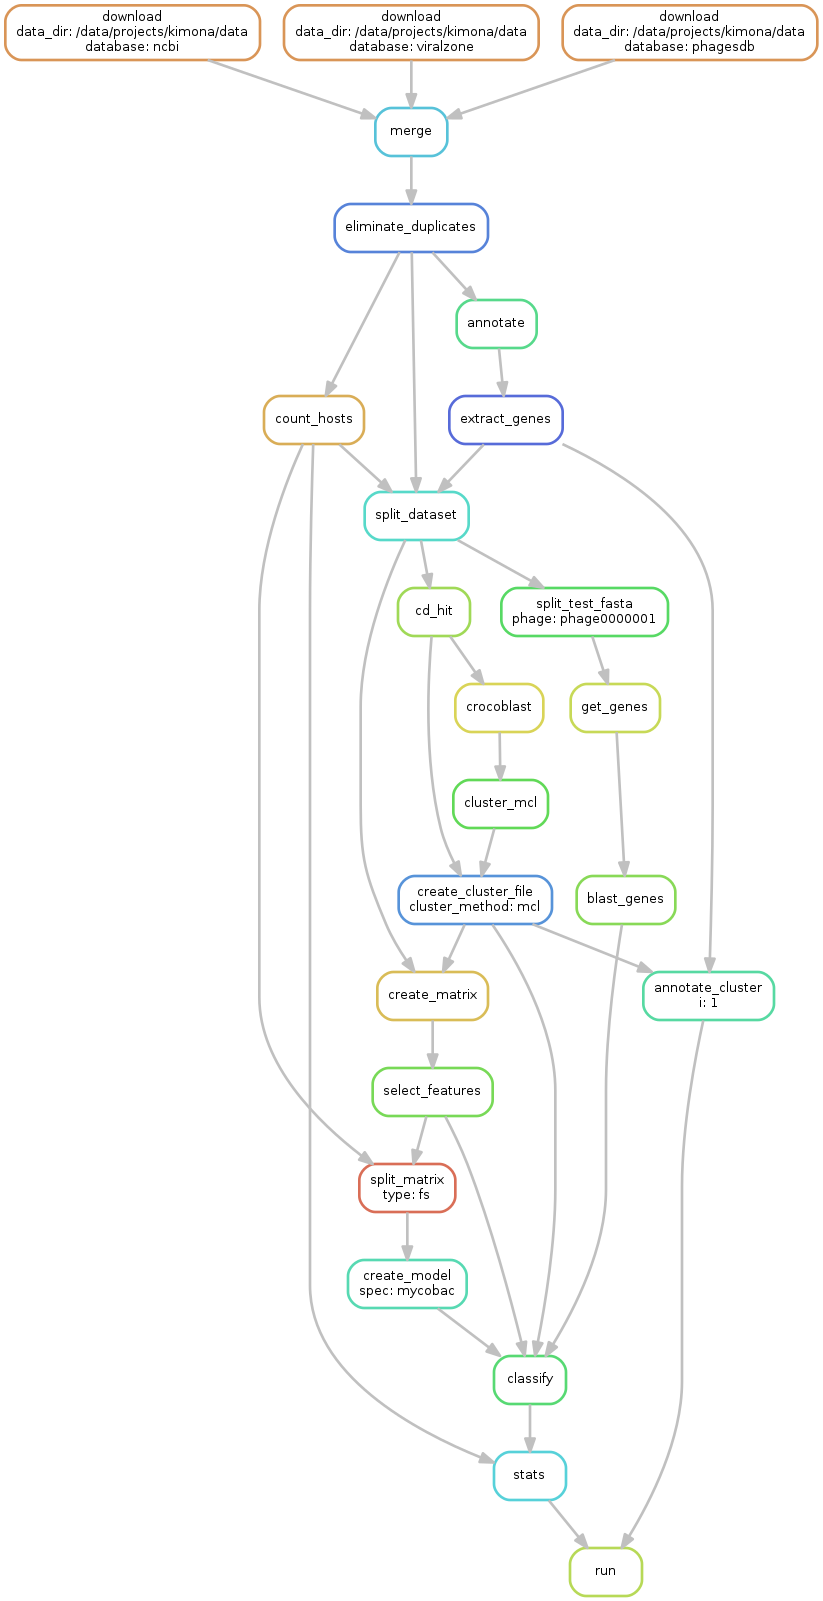
\includegraphics[height=\textheight]{./images/mcl.png}
\centering
\caption{Workflow visualization}
\label{fig:dag}
\end{figure}

\section{Downloading}
Since the first step in our pipeline is downloading of data from publicly available databases, we will provide more detailed description of these sources.
In our pipeline we implemented downloading from three databases.
Although they cover the most of currently sequenced and published phages, we made this step easily extensible for new sources of information.
New source can be added by writing a new download script, naming it \verb|{script_dir}\download_from_{db}.py| and appending this name into variable \verb|DATABASES| in Snakefile. 

\subsection{Downloading from GenBank}
National Center for Biotechnology Information (NCBI) provides an access to GenBank\cite{genbank} database.
This database is a comprehensive source of genomic data with more than 200 million sequences.
Sequences are primarily submitted by individuals all around the globe.
Moreover, GenBank is daily synchronized with European Nucleotide Archive and DNA Data Bank of Japan, which ensures that data are always up-to-date with human knowledge.
NCBI administer GenBank database free of charge and give researchers the possibility to access data through various interfaces as web-based retrieval services, FTP and Entrez\cite{entrez}.
Despite of these facts, there are also shortcomings of using GenBank.
In the time of Next Generation Sequencing the amount of data flowing into GenBank database every day is enormous.
Therefore it is unreasonable to check all data.
This is the cause of redundancy of sequences and sometimes contradictions between information in system.

In our work, data from GenBank was downloaded through our custom script.
We obtained data using python library Biopython \cite{biopython}, which implements python wrapper NCBI Entrez.
Besides, Biopython was also useful for its classes enabling easy manipulation with standard file formats used in bioinformatics.
When downloading sequences, we also created unique identifiers for each record.
Those were used later in pipeline.
Reasons behind the decision to use custom identifiers were ability to remove duplicated sequences and ability to find out possibly multiple sources of each sequence in our dataset.
Downloading from GenBank was our largest source of data with 6704 downloaded records.

\subsection{Downloading from ViralZone}
ViralZone is a website dedicated to viruses. 
It provides highly reliable data about viruses, including bacteriophages.
Information about structure of capsid and genome, life cycle, replication mechanisms, taxonomy, geographical location and host are included.
This website does not store sequences internally, rather it delivers links to RefSeq\cite{refseq} database.
Compared to GenBank, RefSeq database contains fewer sequences, but all of these sequences are curated and manually reviewed.

Our custom script was used to download records from RefSeq database.
Although, large portion of sequences downloaded was identical with GenBank records, some sequences were unique.
Another advantage in performing this action was that it enabled us to pair records in our dataset with full information from ViralZone portal.
By this process we obtained 2107 records. 

% end of session 2018.04.18
% wc chapter* = 32521 letters

\subsection{Downloading from PhagesDB}
PhagesDB is an independent database from NCBI. 
This database is specialized for Actinobacteriophages, so it has less phage records, but it is designed to avoid the time between sequencing and data availability.
Authors declare, at the time of their publication, there was more than 600 records of bacteriophages in phagesdb that were not yet in GenBank.

Furthermore, PhagesDB stores more biological relevant data which are easily obtainable through its RESTful Application Programming Interface.
In our work we used this API to retrieve all genomic sequences with their hosts and annotations.
Eventually we ended up with 2491 phage records from PhagesDB 

\section{Merging and removing of duplicated records}
All download scripts produced four types of output - \verb|<db>.genomes.fasta| \verb|<db>.genomes.conversion| \verb|<db>.genes.fasta| \verb|<db>.genes.conversion|. 
We were aware of high redundancy in our datasets, mainly because many of these records was submitted to more databases at once.
To solve this issue, we merged datasets together and removed duplicated records.
For merging we used standard unix command \verb|cat| for all files with the same type.
For removing duplicated we created our python script.
We looked on all fasta records in merged \verb|genomes.fasta| and if there were more than one with the same sequence, we wrote the one with lesser internal identifier into output fasta file.
We also changed other internal identifiers in files \verb|genomes.conversion| and \verb|genes.conversion| into this identifier.
This approach preserves the relationships between one particular sequence and all data related to it.
Therefore we are able to track phages, based on their internal identifier, to their source databases and also connect them with data already downloaded.
After duplicate removing our dataset consisted of 6277 phage records.

\section{Gene identification}
Despite of downloading annotated sequences with genes, we do not use those genes further in out workflow.
We made this decision because the inconsistency of gene annotations between different databases and different records could be potentially high.
To ensure predictions will be consistent along the entire dataset, we predicted all genes and their annotations by one software - Prokka.
In addition, this software uses regularly updated databases, which guarantee the most up-to-date annotations.
After annotation we extracted all genes with our script.
The output of this program were files \verb|annotated.genes.fasta| and \verb|annotated.genes.conversion| which were further used in pipeline.

\section{Splitting to training set and testing set}
In order to properly evaluate our final models, we divided whole dataset into training set and testing set.
First we find out how many bacteriophages for every group of hosts we have. 
Names of this groups were abreviations of host names.
Reason to use abreviations as group names is that we wanted bring together phages with similar hosts in one group.
We also needed to deal with typos and different formats of the same host.
We selected first 8 groups with the highest counts of records.
These were mycobac, strepto, escheri, gordoni, arthrob, pseudom, lactoco and staphyl with counts 1619, 354, 323, 293, 240, 236, 219, 184 respectively.
All other groups were excluded from our dataset due to insufficient amount of samples.
Furthermore we excluded all phages without the information about their hosts.
This new purified dataset was divided into training set and testing set at a ratio 4:1.
At the end of this step the training set consisted of 2787 records of bacteriophages and the testing set consisted of 699 records.

\section{Alignments}
\section{Local alignment of genes}
After dataset splitting we performed local alignment of the genes in training set against themselves.
Thanks to this step we were able to quantify similarities between different genes, which we needed further in pipeline at clustering step.
The standard bioinformatics tool for this purpose is BLAST \cite{blast}. 
The basic algorithm consists of searching seeds from database on the query sequence and then extending those seeds into neighbouring bases.
This approach provides orders of magnitude faster alignment method than classical Smith-Waterman algorithm \cite{smith_waterman} with comparable sensitivity.
In our pipeline we used software CrocoBLAST \cite{crocoblast}, what is a wrapper around BLAST algorithm which make better use of paralellization than standard BLAST maintained by NCBI.
With CrocoBLAST we were able to reduce time of this local alignment step from four days to one day as opposed to BLAST.
Resulting file was in tab separated format, where first column was gene identifier of query sequence, second column was gene identifier of the target sequence and third column was e-value of alignment. 
E-value is evaluation measure of how similar two sequences are.

\section{Clustering}
Clustering is a problem where we want to determine closely related entities and put them in distinct groups, also called clusters.
In order to be able to distinguish which entity is more closely related to another, we usually use similarity matrix.
To create a similarity matrix we used tab separated file described in previous section.
In this section we will mention different approaches we used for clustering. 
% http://www.paccanarolab.org/scps/
\subsection{Markov Cluster Algorithm}
First approach we used was Markov Cluster Algorithm. 
We used already implemented version called mcl \cite{mcl}.
This software is often used in bioinformatics for clustering of sequences based on their similarity.
It has the capability to determine number of resulting clusters automatically and except input data, it requires only one parameter.
This parameter is called inflation and usually takes float number values from 1.2 to 5.0.
Smaller values results in less and bigger clusters.
In our work we needed as few clusters as possible, mainly due to number of phage records in our dataset.
In case of too many clusters we would have too many features for classifier and we would risk overfitting of our final models to training dataset.
For these reasons we used inflation value 1.2, which created 15017 clusters.

\subsection{Markov Cluster Algorithm with global alignment}
To get more accurate clustering we tried different approach, where we determined similarity score of alignments with needleman-wunsch algorithm. \cite{needleman-wunsch}
This algorithm is able to calculate best global alignment score of given protein sequences.
The difference between global alignment and local alignment is that former aligns sequences from end to end.
The resulting score was then used as input to mcl algorithm described in previous section.
By this approach we created 9176 final clusters.

\subsection{Spectral clustering}
Spectral clustering is different algorithm used for clustering.
In this work we tried SCPS implementation\cite{scps}.
Authors of this bioinformatics software declare quality of clusters quantified by a measure that combines sensitivity and specificity to be better by 28\% in comparison to mcl algorithm.
Unfortunately, memory required by this program was too high and we were not able to run it on our server with all input data. 

\section{Cluster annotation}
Created clusters were further annotated to examine their functions.
We expected that proteins with similar function will end up in the same cluster. 
This was mostly the case although the information about particular proteins were sparse with a lot of proteins without any information in database.
For annotation we used software interproscan\cite{interpro}.
This tool scans given protein sequences against the protein signatures in databases PROSITE, PRINTS, Pfam, ProDom and SMART.
% is supported by our knowledge of phage biology

\section{Creation of matrix}
Probably the most important part of our pipeline is binary matrix created from phage records and clusters.
For the purpose of matrix creation we wrote our own script.
This script takes as input tree files - \verb|annotated.genes.conversion|, \verb|genes.clstr| and \verb|genomes.list|.
The first file is needed in order to know which phage contains which particular gene.
The second file is file containing gene clusters in tab separated format where each line represents one cluster.
The last file is just a list of all phages which should be included in matrix.
This script is also parallelized to enable use of multiple computational nodes.
We created raw matrix with 2787 rows representing phage records and 15017 columns represented gene clusters.
This matrix was further reduced with feature selection method Variance Threshold.
During this process we removed all columns with ones or zeroes in more than 99\%.
The removed columns have a high potential to be non-functional proteins which created its own clusters.
After feature selection our matrix contained 2787 phage records and 1818 distinct gene clusters.
This matrix was used as input to machine learning algorithms. 


